\node[inner sep=0pt] (alice) at (0,0)
    {
\includegraphics[width=.25\textwidth]{../pictures/examples/alice.jpeg}};
\node[inner sep=0pt] (bob) at ($(alice) + (6,0)$)
    {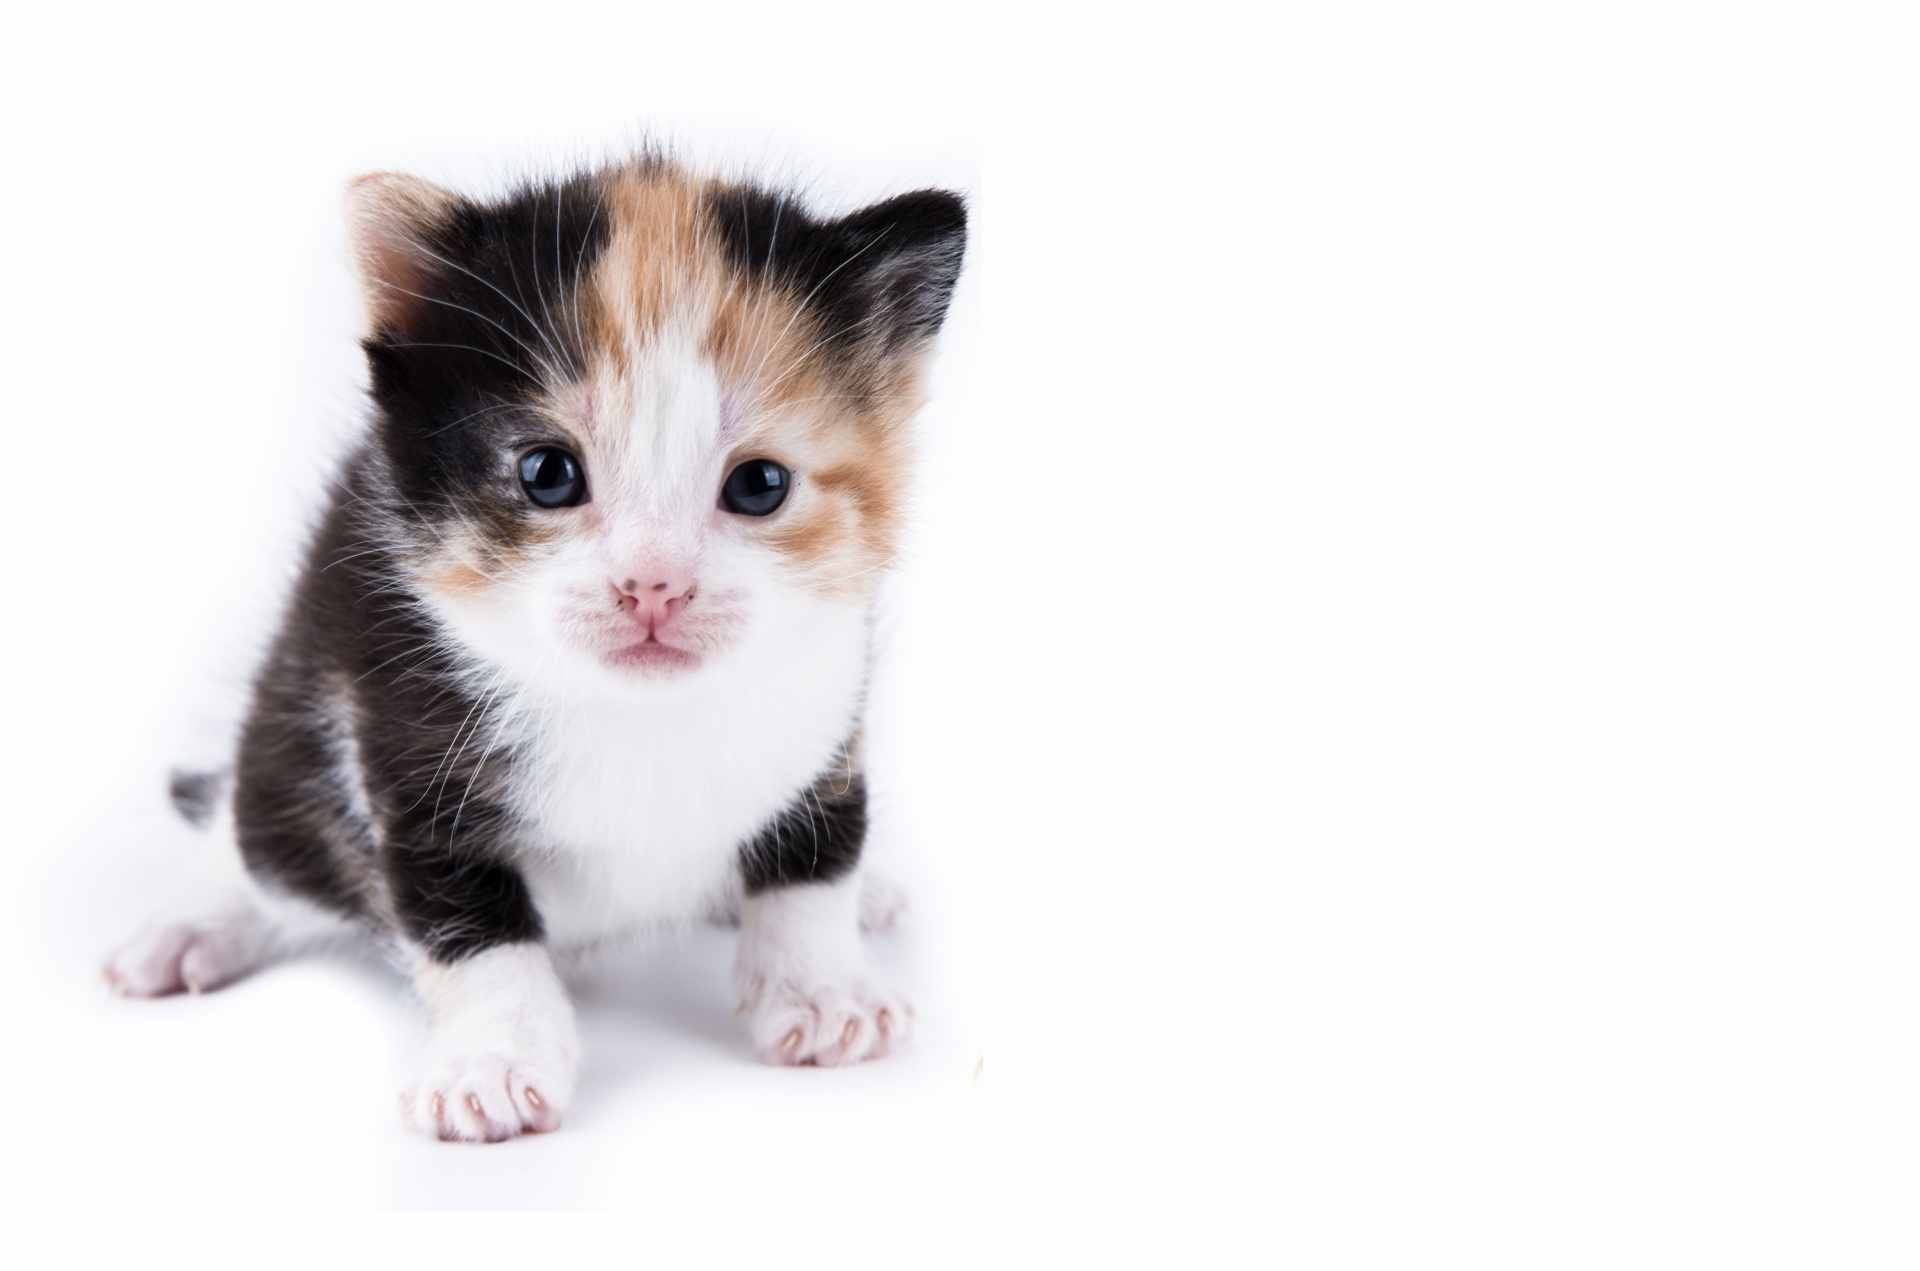
\includegraphics[width=.25\textwidth]{../pictures/examples/bob.jpeg}};
\node[inner sep=0pt] (eve) at ($(alice) + (3,2)$)
    {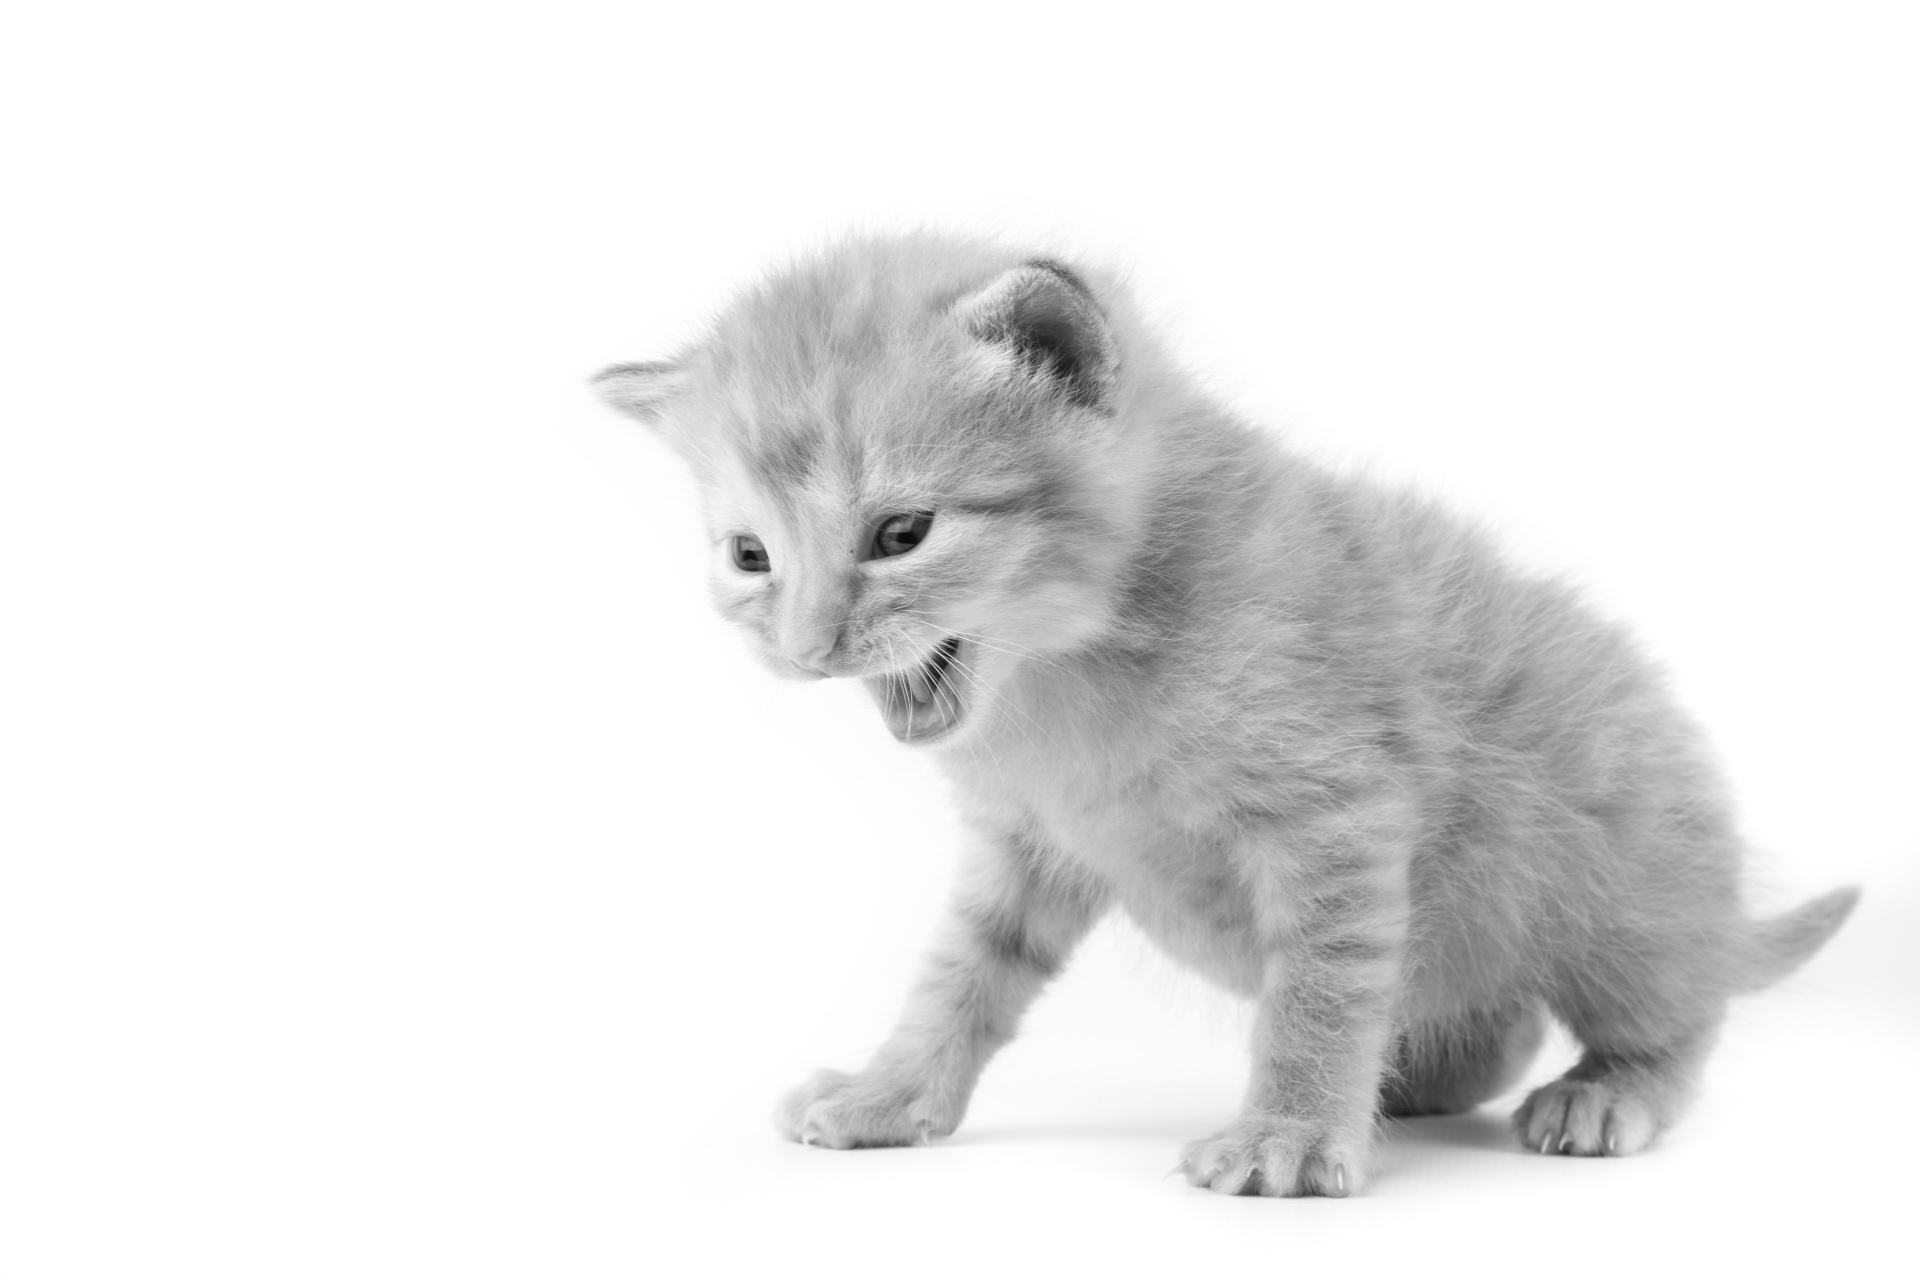
\includegraphics[width=.25\textwidth]{../pictures/examples/eve.jpg}};
\node[inner sep=0pt] (alicec) at ($(alice) + (-1,0)$)
    {
\includegraphics[width=.10\textwidth]{../pictures/examples/computer.jpg}};
\node[inner sep=0pt] (bobc) at ($(bob) + (1,0)$)
    {
\includegraphics[width=.10\textwidth]{../pictures/examples/computer.jpg}};
\node  at ($(bob) + (1.2,-1)$)
    {\tiny déchiffrement\_AES.c};
\node at ($(alice) + (-1,-1)$)
{\tiny chiffrement\_AES.c};

\node[color = red] at ($(alice) + (-1,0.2)$) {M};
\node[color = red] at ($(bob) + (1,0.2)$) {\tiny $E_k(M)$};

\node[color = red] (C) at ($(alice) + (3,0.5)$) {\small$E_k(M)$};

\draw[->, thick] (alice) -- (bob);
